\section{特殊的几种函数}

\subsection{常考构造 $\frac{lnx}{x}$}

\begin{theorem}[函数 $\frac{\ln x}{x}$ 的性质]
    \begin{itemize}
        \item \textbf{单调性}: 函数 $f(x) = \frac{\ln x}{x}$ 在 $(0, e)$ 上单调递增，在 $(e, +\infty)$ 上单调递减。
        \item \textbf{极限值}: 并且当 $x \to 0^+$ 时，$f(x) \to -\infty$；当 $x \to +\infty$ 时，$f(x) \to 0+$.
        \item \textbf{零点}: 函数在 $(0, +\infty)$ 上有唯一零点 $x = 1$.
        \item \textbf{值相等}: $\frac{ln4}{4} = \frac{ln2}{2}$.
    \end{itemize}
\end{theorem}

\begin{example}
    已知函数 $f(x)=\frac{\ln x}{x}+2$ ，则（\quad）
    \begin{tasks}(4)
        \task $f(x)$ 在 $(0, \mathrm{e})$ 上单调递增
        \task $f(\mathrm{e})>f(3)>f(2)$
        \task $f(x)$ 的最大值为 $\mathrm{e}+2$
        \task $f(x)$ 有唯一零点
    \end{tasks}
\end{example}

\v{12em}

\begin{example}[变式 $\frac{lnx}{x^n}$]
    已知函数 $f(x)=\ln x-a x^2$ ．
    \begin{enumerate}
        \item 当 $a=1$ 时，求 $f(x)$ 的最大值；

        \item 若 $\forall x \in(0,+\infty), ~ f(x)<0$ ，求实数 $a$ 的取值范围．
    \end{enumerate}
\end{example}

\begin{example}
    已知函数 $f(x)=\ln x-a x^2$ ．
    \begin{itemize}
        \item 当 $a=1$ 时，求 $f(x)$ 的最大值；
        \item 若 $\forall x \in(0,+\infty), ~ f(x)<0$ ，求实数 $a$ 的取值范围．
    \end{itemize}
\end{example}

\subsubsection{比较大小}

\begin{problem}
\begin{itemize}
    \item 试比较 $\pi^e$ 和 $e^\pi$ 的大小。
    \item 试比较 $2025^{2026}$ 和 $2026^{2025}$ 的大小。
\end{itemize}
\end{problem}

\v{12em}

\begin{example}
    已知 $a=\frac{4(2-\ln 4)}{e^2}, b=\frac{1}{e}, c=\frac{\ln 4}{4}$ ，其中 $e$ 为自然对数的底数，则 $a, b, c$ 的大小关系为（\quad）
    \begin{tasks}(4)
        \task $a<c<b$
        \task $c<a<b$
        \task $a<b<c$
        \task $b<a<c$
    \end{tasks}
\end{example}

\v{12em}

\begin{example}
    （2022 吉林高二期末）下列命题为真命题的有（\quad）
    \begin{tasks}(4)
        \task $\ln 3<\sqrt{3} \ln 2$ ；
        \task $\ln \pi<\sqrt{\frac{\pi}{\mathrm{e}}}$ ；
        \task $2^{\sqrt{15}}<15$ ；
        \task $3 e \ln 2>4 \sqrt{2}$ ．
    \end{tasks}
\end{example}

\v{12em}

\begin{example}
    （2021 陕西汉中高二期末）已知 $a, b, c \in (0, \mathrm{e})$，$a \ln 5=5 \ln a, b \ln 6= 6 \ln b, c \ln 7=7 \ln c$ ，则 （ \quad）
    \begin{tasks}(4)
        \task $a>c>b$
        \task $a>b>c$
        \task $c>a>b$
        \task $c>b>a$
    \end{tasks}
\end{example}

\v{12em}

\begin{example}
    （2022 四川省资阳中学高二期末）若 $a=\frac{\ln 2}{2}, b=\frac{1}{\mathrm{e}}, c=\frac{2 \ln 3}{9}$ ，则（\quad ）
    \begin{tasks}(4)
        \task $b>a>c$
        \task $b>c>a$
        \task $a>b>c$
        \task $a>c>b$
    \end{tasks}
\end{example}

\v{12em}

\subsection{大题存在的形式}

\begin{example}
    (2021 全国甲卷 21 题)
    已知：$a>0, a \neq 1, f(x)=\frac{x^a}{a^x}(x>0)$
    \begin{itemize}
        \item 若 $a=2$ ，求 $f(x)$ 单调区间
        \item 若曲线 $y=f(x)$ 与直线 $y=1$ 有且仅有 2 个交点，求 $a$ 的取值范围
    \end{itemize}
\end{example}

\v{10em}

\subsection{六大母函数的图像与特征}

\begin{center}
    \begin{tabular}{|c|c|c|}
        \hline
        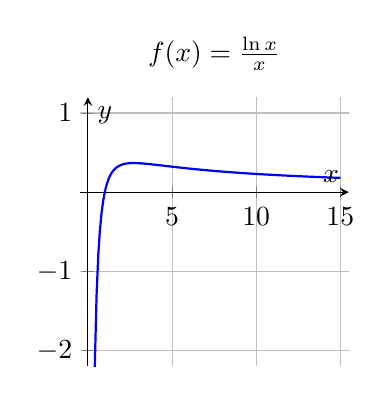
\begin{tikzpicture}
            \begin{axis}[
                    width=5cm, height=5cm,   % 设置每个图的大小
                    title={$f(x) = \frac{\ln x}{x}$}, % 标题
                    xlabel=$x$, ylabel=$y$,       % 坐标轴标签
                    axis lines=middle,              % 坐标轴在中间
                    grid=major,                     % 显示主网格
                    xmin=0, xmax=15,                % X轴范围
                    ymin=-2, ymax=1,                % Y轴范围
                    enlarge x limits={abs=0.5},     % X轴留白
                    enlarge y limits={abs=0.2},     % Y轴留白
                    legend pos=south east,           % 图例位置
                    restrict y to domain=-5:10
                ]
                \addplot[
                    blue, thick,                    % 蓝色粗实线
                    samples=150,                    % 采样点数，越多越平滑
                    domain=0.01:15                  % 绘图定义域
                ] {ln(x)/x};
            \end{axis}
        \end{tikzpicture}
         &

        % --- 图 2: f(x) = x / ln(x) ---
        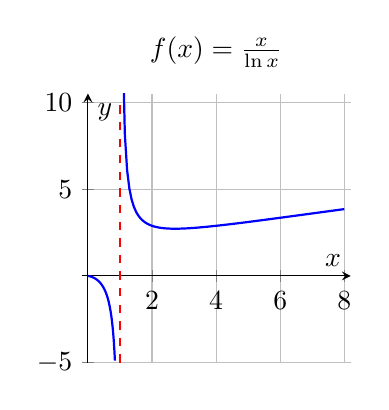
\begin{tikzpicture}
            \begin{axis}[
                    width=5cm, height=5cm,
                    title={$f(x) = \frac{x}{\ln x}$},
                    xlabel=$x$, ylabel=$y$,
                    axis lines=middle,
                    grid=major,
                    xmin=0, xmax=8,
                    ymin=-5, ymax=10,
                    enlarge x limits={abs=0.2},
                    enlarge y limits={abs=0.5, upper},
                    restrict y to domain=-5:
                ]
                % 绘制 (0, 1) 区间的左侧分支
                \addplot[blue, thick, samples=100, domain=0.01:0.99] {x/ln(x)};
                % 绘制 (1, +inf) 区间的右侧分支
                \addplot[blue, thick, samples=100, domain=1.01:8] {x/ln(x)};
                % 绘制渐近线
                \draw[red, dashed] (1, -5) -- (1, 10);
            \end{axis}
        \end{tikzpicture}
         &

        % --- 图 3: f(x) = x * ln(x) ---
        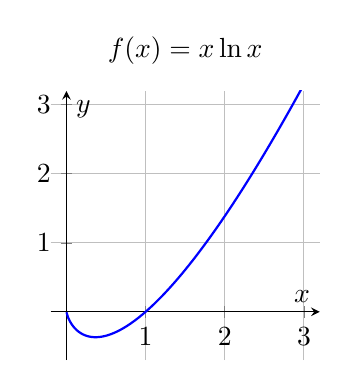
\begin{tikzpicture}
            \begin{axis}[
                    width=5cm, height=5cm,
                    title={$f(x) = x \ln x$},
                    xlabel=$x$, ylabel=$y$,
                    axis lines=middle,
                    grid=major,
                    xmin=0, xmax=3,
                    ymin=-0.5, ymax=3,
                    enlarge x limits={abs=0.2},
                    enlarge y limits={abs=0.2},
                    restrict y to domain=-5:10
                ]
                \addplot[blue, thick, samples=150, domain=0.001:3] {x*ln(x)};
            \end{axis}
        \end{tikzpicture}
        \\ % 结束第一行

        \hline

        % --- 图 4: f(x) = x * e^x ---
        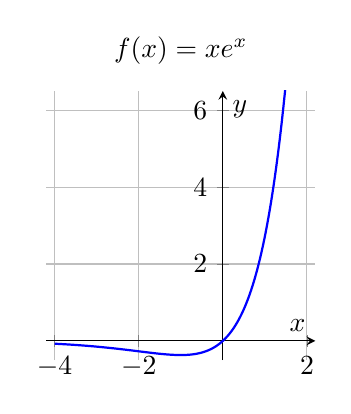
\begin{tikzpicture}
            \begin{axis}[
                    width=5cm, height=5cm,
                    title={$f(x) = x e^x$},
                    xlabel=$x$, ylabel=$y$,
                    axis lines=middle,
                    grid=major,
                    xmin=-4, xmax=2,
                    ymin=-0.5, ymax=6,
                    enlarge x limits={abs=0.2},
                    enlarge y limits={abs=0.5, upper}
                ]
                \addplot[blue, thick, samples=150, domain=-4:2] {x*exp(x)};
            \end{axis}
        \end{tikzpicture}
         &

        % --- 图 5: f(x) = e^x / x ---
        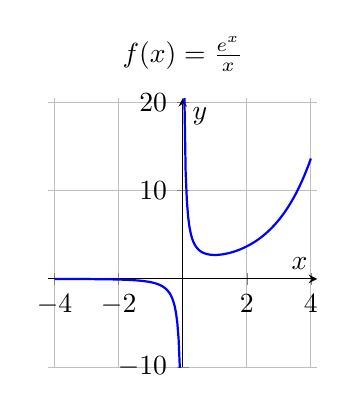
\begin{tikzpicture}
            \begin{axis}[
                    width=5cm, height=5cm,
                    title={$f(x) = \frac{e^x}{x}$},
                    xlabel=$x$, ylabel=$y$,
                    axis lines=middle,
                    grid=major,
                    xmin=-4, xmax=4,
                    ymin=-10, ymax=20,
                    enlarge x limits={abs=0.2},
                    enlarge y limits={abs=0.5, upper}
                ]
                % 绘制 x < 0 的左侧分支
                \addplot[blue, thick, samples=100, domain=-4:-0.05] {exp(x)/x};
                % 绘制 x > 0 的右侧分支
                \addplot[blue, thick, samples=100, domain=0.05:4] {exp(x)/x};
            \end{axis}
        \end{tikzpicture}
         &

        % --- 图 6: f(x) = x / e^x ---
        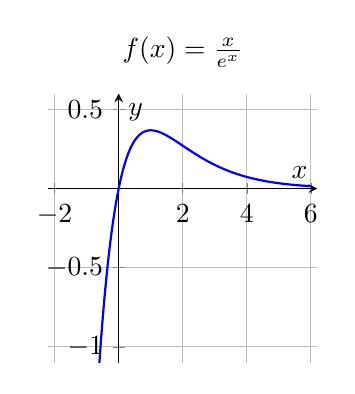
\begin{tikzpicture}
            \begin{axis}[
                    width=5cm, height=5cm,
                    title={$f(x) = \frac{x}{e^x}$},
                    xlabel=$x$, ylabel=$y$,
                    axis lines=middle,
                    grid=major,
                    xmin=-2, xmax=6,
                    ymin=-1, ymax=0.5,
                    enlarge x limits={abs=0.2},
                    enlarge y limits={abs=0.1}
                ]
                \addplot[blue, thick, samples=150, domain=-2:6] {x/exp(x)};
            \end{axis}
        \end{tikzpicture}
        \\ % 结束第二行
        \hline
    \end{tabular}
\end{center}